\documentclass[draft]{article}

\usepackage[utf8]{inputenc}
\usepackage[T1]{fontenc}
\usepackage[francais]{babel}

\usepackage{multicol}

\usepackage[demo]{graphicx}
\graphicspath{ {images/} }

\usepackage{enumitem}

\usepackage{amssymb}
\usepackage{amsthm}
\usepackage{amsmath}

\newtheorem*{myNot}{Notation}
\newtheorem{myDef}{Definition}

\theoremstyle{definition}
\newtheorem{myRem}{Remarque}

\title{Résumé du mémoire de maîtrise de Florian \bsc{Tramèr}}
\author{François \bsc{Bidet}}

\begin{document}

\maketitle

%%%%%%%%%%%%%%%%%%%%%%%%%%%%%%
%        Présentation        %
%%%%%%%%%%%%%%%%%%%%%%%%%%%%%%

\section{Présentation}

Ce document regroupe des définitions et considérations extraites de mémoire de master ``Algorithmic Fairness Revisited'' de Florian Tramèr.

%%%%%%%%%%%%%%%%%%%%%%%%%%%%%%
%         Notations          %
%%%%%%%%%%%%%%%%%%%%%%%%%%%%%%

\section{Notations}

\begin{myNot}
  Un algorithme est noté $\mathcal{A}$.
\end{myNot}

\begin{myNot}
  On note $N$ le taille du dataset.
\end{myNot}

\begin{myNot}
  Les données collectées d'un utilisateur sont notées $X \in \mathcal{X}$.
\end{myNot}

\begin{myNot}
  L'ensemble des résultats d'un algorithme est noté $\mathcal{O}$ et une sortie particulière est notée $o \in \mathcal{O}$.
\end{myNot}

\begin{myNot}
  Les attributs protégés (ou sensibles) sont notés $S$.

  Si $S$ est binaire, on appelle $s^{+}$ la valeur pour laquelle l'algorithme favorise et $s^{-}$ celle pour laquelle il défavorise.
\end{myNot}

\begin{myNot}
  Une estimation par rapport aux données d'une probabilité $P$ est notée $\hat{P}$.
\end{myNot}

\begin{myNot}
  La fonction d'utilité d'un utilisateur est notée $U \in \mathcal{U}$.
\end{myNot}

\begin{myNot}
  On note les attributs non protégés nécessaires à un travail (business) $B \in \mathcal{B}$.
  On note les classes d'utilisateurs nécessaires à un travail $K \in \mathcal{K}$.
  Un business fournit une fonction d'association $h : \mathcal{B}^{n} \rightarrow \mathcal{K}^{n}$ pour tout $n \geq 1$.
\end{myNot}


%%%%%%%%%%%%%%%%%%%%%%%%%%%%%%
%          Mesures           %
%%%%%%%%%%%%%%%%%%%%%%%%%%%%%%

\section{Mesures d'équité}

\begin{myDef}
  \label{defSimple}
  Un algorithme est juste/équitable si sa sortie est indépendante des attributs protégés.
\end{myDef}

\begin{myDef}
  Pour un attribut protégé $S \in \{s^+, s^-\}$, respectivement favorisé et défavorisé pour la même sortie $o \in \mathcal{O}$, on définit la mesure ``selection-lift'' :
  \[
  slift(s^+;o) = \frac{\hat{P}(o|s^+)}{\hat{P}(o|s^-)}
  \]
\end{myDef}

\begin{myDef}
  Pour un attribut protégé $S \in \{s^+, s^-\}$, respectivement favorisé et défavorisé pour la même sortie $o \in \mathcal{O}$, on définit la mesure ``difference-based selection-lift'' :
  \[
  slift_{d}(s^+;o) = \hat{P}(o|s^+) - \hat{P}(o|s^-)
  \]
\end{myDef}

\begin{myDef}[$a$-protection]
  Pour une mesure d'équité $f(.)$ et un seuil fixé $a \in \mathbb{R}$, on dit que $\mathcal{A}$ est ``$a$-protecteur'' par rapport à $f(.)$, $s^{+} \in \mathcal{S}$ et $o \in \mathcal{O}$ si $f(s^{+},o) < a$. Sinon, $\mathcal{A}$ est dit ``$a$-discriminant'' ou ``$a$-discriminatoire''.

  Soit $\left[ L_{1} , L_{2} \right]$ l'intervalle de confiance de $f(s^{+},o)$ au niveau de signification $\beta$, alors :
  \begin{itemize}
  \item $\mathcal{A}$ est $a$-protecteur au niveau de signification $\beta$ si $L_{2} < a$
  \item $\mathcal{A}$ est $a$-discriminant au niveau de signification $\beta$ si $L_{1} \geq a$
  \end{itemize}
\end{myDef}

\begin{myDef}[Mesures théoriques de l'information]
  La divergence de Kullback-Leibler entre $\hat{P}(S)$ et $\hat{P}(S|O = o)$ est définie par
  \[
  D_{KL}(\hat{P}(S|O=o) || \hat{P}(S)) = \sum_{s} \hat{P}(s|o) \ln \left( \frac{\hat{P}(s|o)}{\hat{P}(s)} \right)
  \]
\end{myDef}

\begin{myDef}[Parité statistique]
  Un algorithme statisfait empiriquement la parité statistique jusqu'au biais $\epsilon$ si
  \[
  D_{TV}( \hat{P}(O|S=s^{+}), \hat{P}(O|S=s^{-})) = \frac{1}{2} \sum_{o \in \mathcal{O}} \left| \hat{P}(o|s^{+}) - \hat{P}(o|s^{-}) \right| \leq \epsilon
  \]
  où $D_{TV}(P,Q)$ est la distance de variation totale entre les distributions $P$ et $Q$.
\end{myDef}

\begin{myDef}[Information mutuelle (MI)]
  L'information mutuelle empirique entre $S$ et $O$ est définie par
  \[
  \hat{I}(S;O) = \mathbb{E}_{O} \left[ D_{KL}(\hat{P}(S|O=o) || \hat{P}(S)) \right] = \sum_{s \in \mathcal{S}} \sum_{o \in \mathcal{O}} \hat{P}(s,o) \ln \left( \frac{\hat{P}(s,o)}{\hat{P}(s) \hat{P}(o)} \right)
  \]

  On définit de même l'information mutuelle empirique normalisée entre $S$ et $O$ par
  \[
  \hat{I}_{norm}(S;O) = \frac{\hat{I}(S;O)}{min\{ \hat{H}(S), \hat{H}(O) \}} \in \left[ 0, 1 \right]
  \]
  où $\hat{H}(Y)$ est l'entropie empirique d'une variable aléatoire $Y$ : \[\hat{H}(Y) = - \sum_{y} \hat{P}(Y=y) \ln \hat{P}(Y=y)\]
\end{myDef}

\begin{myDef}[MI-équité]
  Un algorithme satisfait l'équité $\epsilon$-MI par rapport à l'attribut protégé $S$ si $\hat{I}(S;O) \leq \epsilon$.
  De même, un algorithme satisfait l'équité $\epsilon$-MI normalisée par rapport à l'attribut protégé $S$ si $\hat{I}_{norm}(S;O) \leq \epsilon$.
\end{myDef}

\begin{myDef}[équité statistique générique]
  Soit $p$ la p-value obtenue par un test statistique pour l'hypothèse nulle $S \bot O$. Alors $\mathcal{A}$ est statistiquement juste\slash équitable par rapport à $S$ au niveau de signification $\beta$ si $p \leq \beta$.
\end{myDef}

\begin{myDef}[``User-Utilitarian Fairness'']
  $\mathcal{A}$ est juste par rapport à un attribut protégé $S$ et à une fonction d'utilité $U$ si et seulement si $U \bot S$.
\end{myDef}

\begin{myDef}[``Business-Utilitarian Fairness'']
  \label{defBusiness}
  $\mathcal{A}$ est juste par rapport à un attribut protégé $S$ et à une classe $K$ si et seulement si
  \begin{enumerate}
  \item Il existe un ensemble d'attributs $\mathcal{B}$ et une association $h : \mathcal{B}^{n} \rightarrow \mathcal{K}^{n}$ qui sont une représentation valide des nécessités d'un travail
  \item $O \bot S | K$
  \end{enumerate}
\end{myDef}

\begin{myDef}[Information mutuelle conditionnelle]
  L'information mutuelle conditionnelle entre $S$ et $O$ sachant $K$ est définie par
  \[
  \hat{I}(S;O|K) = \mathbb{E}_{K}[\hat{I}(S;O)|K] = \sum_{k \in \mathcal{K}} \hat{P}(k) \sum_{s \in \mathcal{S}} \sum_{o \in \mathcal{O}} \hat{P}(s,o|k) \ln \left( \frac{\hat{P}(s,o|k)}{\hat{P}(s|k) \hat{P}(o|k)} \right)
  \]
  La mesure normalisée $\hat{I}_{norm}(S;O|K)$ est donnée par $\frac{\hat{I}(S;O|K)}{\min \left\{ \hat{H}(S|K), \hat{H}(O|K) \right\}}$.
\end{myDef}

La définition du ``G-test'' est une définition qui n'est pas créée par l'auteur. ``G-test'' est une évaluation statistique populaire de la qualité d'une hypothèse.
\begin{myDef}[G-test]
  Pour chaque paire $(s,o) \in \mathcal{S} \times \mathcal{O}$, on note le nombre d'observation $f_{s,o}$. Alors le G-test est donné par
  \[
  G = 2 \sum_{s \in \mathcal{S}} \sum_{o \in \mathcal{O}} f_{s,o} \ln \left( \frac{f_{s,o}}{E_{s,o}} \right)
  \]
  où $E_{s,o}$ est la fréquence d'observation théorique si l'hypothèse nulle est valide.
\end{myDef}

\begin{myDef}[G-test conditionnel]
  Avec $f_{s,o,k}$ le nombre d'observation du triplet $(s,o,k)$ et $E_{s,o,k}$ le nombre théorique si l'hypothèse nulle est valide, le G-test est donné par
  \[
  G_{K} = 2 \sum_{s \in \mathcal{S}} \sum_{o \in \mathcal{O}} \sum_{k \in \mathcal{K}} f_{s,o,k} \ln \left( \frac{f_{s,o,k}}{E_{s,o,k}} \right)
  \]
\end{myDef}


%%%%%%%%%%%%%%%%%%%%%%%%%%%%%%
%      Remarques Auteur      %
%%%%%%%%%%%%%%%%%%%%%%%%%%%%%%

\section{Remarques dans le document}

\subsection{Remarques sur les mesures}

\begin{myRem}
  Pour un attribut protégé binaire $S \in {s^{+}, s^{-}}$, on a :
  \begin{align*}
    \hat{P}(S,O) = \hat{P}(S) \hat{P}(O)
    &\Longleftrightarrow slift(s^{+};o) = 1, \forall o \in \mathcal{O} \\
    &\Longleftrightarrow slift_{d}(s^{+};o) = 0, \forall o \in \mathcal{O} \\
    &\Longleftrightarrow D_{KL}(\hat{P}(S|O = o) || \hat{P}(S)) = 0, \forall o \in \mathcal{O}
  \end{align*}
\end{myRem}

\begin{myRem}[Asymétrie]
  Les mesures de ``selection-lift'' ne sont pas symétriques. En général
  \[
  slift(s^{+};o) \neq slift(s^{-};o)
  \]
  et
  \[
  slift_{d}(s^{+};o) \neq slift_{d}(s^{-};o)
  \]
\end{myRem}

\begin{myRem}[lien entre G-test et information mutuelle]
  Le G-test vérifie
  \[
  G = 2 \cdot N \cdot \hat{I}(S;O)
  \]
\end{myRem}

\begin{myRem}[lien entre G-test et information mutuelle conditionnelle]
  Le G-test vérifie
  \[
  G_{K} = 2 \cdot N \cdot \hat{I}(S;O|K)
  \]
  avec $E_{s,o,k} = N \cdot \hat{P}(k) \hat{P}(s|k) \hat{P}(o|k)$
\end{myRem}

\begin{myRem}
  Le G-test dépend de la taille du dataset : plus le dataset est grand, plus l'amplitude du G-test peut être importante.
\end{myRem}

\subsection{Considérations}

\begin{myRem}
  Un certain nombre de mesures d'équité ne prennent pas en compte la taille des catégories, ce qui peut mener à des contradiction : un résultat peut être annoncé comme peu biaisé alors qu'il y a un énorme biais sur une très petite population.

  \begin{multicols}{2}
    \begin{tabular}{l|r|r}
      $\mathcal{A}$ & Homme & Femme \\
      \hline
      Président & 20 & 5 \\
      Manager & 9 980 & 9 995 \\
      Employé & 10 000 & 10 000 \\
    \end{tabular}
    \[
    D_{TV} = 7.50 \cdot 10^{-4}
    \]
    \[
    \hat{I}_{norm} = 1.74 \cdot 10^{-4}
    \]

    \columnbreak

    \begin{tabular}{l|r|r}
      $\mathcal{A}$ & Homme & Femme \\
      \hline
      Président & 20 & 20 \\
      Manager & 9 970 & 9 995 \\
      Employé & 10 010 & 9 985 \\
    \end{tabular}
    \[
    D_{TV} = 1.25 \cdot 10^{-3}
    \]
    \[
    \hat{I}_{norm} = 1.13 \cdot 10^{-6}
    \]
  \end{multicols}
\end{myRem}

\begin{myRem}
  On ne peut pas observer un biais sur des catégories en convertissant en donnée binaire.
  Exemple, la discrimination envers les personnes noires n'apparaît pas :

  \begin{tabular}{c c@{\extracolsep{1em}}c c@{\extracolsep{1em}}c c}
    \multicolumn{6}{c}{$S$}
    \\
    \hline
    \multicolumn{2}{c}{Black} & \multicolumn{2}{c}{White} & \multicolumn{2}{c}{Hispanic}
    \\
    \cline{1-2}
    \cline{3-4}
    \cline{5-6}
    Applicants & Hired
    &
    Applicants & Hired
    &
    Applicants & Hired
    \\
    100 & 50\%
    &
    100 & 80\%
    &
    100 & 20\%
    \\
    \\
    \multicolumn{6}{c}{S'}
    \\
    \hline
    \multicolumn{2}{c}{Black} & \multicolumn{4}{c}{Not Black}
    \\
    \cline{1-2}
    \cline{3-6}
    Applicants & Hired
    &
    \multicolumn{2}{c}{Applicants} & \multicolumn{2}{c}{Hired}
    \\
    100 & 50\%
    &
    \multicolumn{2}{c}{200} & \multicolumn{2}{c}{50\%}
    \\
    \\
  \end{tabular}

  Le biais envers les personnes noires n'apparaît pas car la favorisation des personnes blanches est compensée par la discrimination envers les personnes hispaniques.
\end{myRem}

\begin{myRem}[Justification ``business-utilitarian fairness'']
  Considérons le cas d'un recrutement de 120 employés avec les candidats répartis comme suit :
  \[
  \begin{tabular}{l r r}
    & Male & Female \\
    \hline
    PhD & 60 & 24 \\
    Master & 240 & 156 \\
    Bachelor & 150 & 270 \\
  \end{tabular}
  \]

  \begin{enumerate}
  \item On peut considérer que le niveau Master est le niveau minimal à avoir pour pouvoir être embauché.
    On définit alors
    \[
    \mathcal{K} = \left\{ qualified, non \text{-} qualified \right\}
    \]
    \[
    B \in \left\{ PhD, Master, Bachelor \right\}
    \]
    et
    \[
    h(B) = qualified \Longleftrightarrow B \in \left\{ PhD, Master \right\}
    \]
    On a alors 120 postes pour 480 candidats qualifiés, ce qui fait 25\% des candidats à embaucher :
    \[
    \begin{tabular}{l r r@{\extracolsep{1em}}r r}
      & \multicolumn{2}{c}{Male} & \multicolumn{2}{c}{Female}
      \\
      \cline{2-3}
      \cline{4-5}
      & Applicants & Hired & Applicants & Hired
      \\
      \hline
      PhD & 60 & 25\% & 24 & 25\%
      \\
      Master & 240 & 25\% & 156 & 25\%
      \\
      Bachelor & 150 & 0\% & 270 & 0\%
      \\
      \hline
      Total & 450 & 16.7\% & 450 & 10\%
      \\
    \end{tabular}
    \]

  \item On peut considérer que l'on désire les employés les plus qualifiés.
    On définit alors
    \[
    \mathcal{K} = \left\{ most \text{-} qualified, qualified, non \text{-} qualified \right\}
    \]
    On embauche alors l'ensemble des candidats de niveau doctorat et 36 des 396 candidats de niveau Master, avec le cas favorable où 21 des 240 hommes et 15 des 156 femmes de niveau Master sont embauchés :
    \[
    \begin{tabular}{l r r@{\extracolsep{1em}}r r}
      & \multicolumn{2}{c}{Male} & \multicolumn{2}{c}{Female}
      \\
      \cline{2-3}
      \cline{4-5}
      & Applicants & Hired & Applicants & Hired
      \\
      \hline
      PhD & 60 & 100\% & 24 & 100\%
      \\
      Master & 240 & 9\% & 156 & 9\%
      \\
      Bachelor & 150 & 0\% & 270 & 0\%
      \\
      \hline
      Total & 450 & 18\% & 450 & 8.7\%
      \\
    \end{tabular}
    \]
  \end{enumerate}

  Les résultats présentent donc une discrimination d'après la définition \ref{defSimple} mais sont ``justes'' d'après la définition \ref{defBusiness} si les ensembles $\mathcal{K}$ sont acceptés.
\end{myRem}

\begin{myRem}[Classifieur à deux étages]
  Pour effectuer une classification qui est juste par rapport à des exigences de l'entreprise, on peut concevoir un classifieur en deux niveaux comme suit :
  \begin{center}
    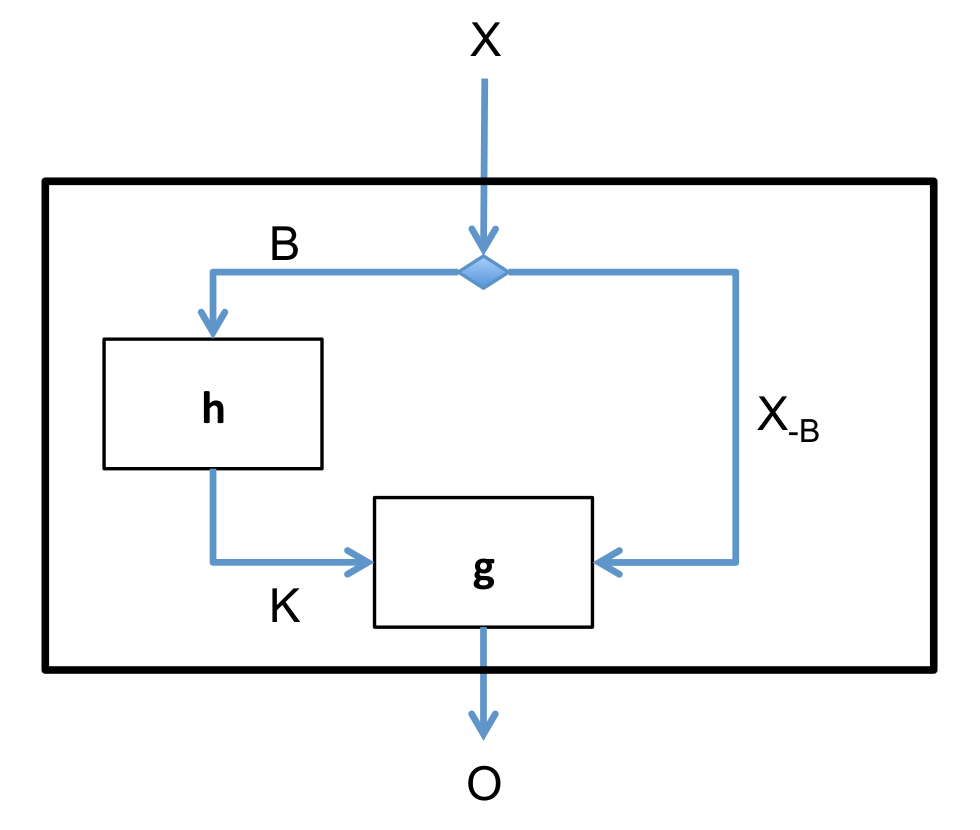
\includegraphics[width=0.7\textwidth]{twoStageClassifier}
  \end{center}
  On définit une première fonction $h$ qui associe un profile d'attributs $B$, nécessaires à l'entreprise, à une classe $K$ puis une deuxième fonction $g$ effectue la classification en fonction de la classe $K$ et du profile privé des attributs $B$. C'est cette dernière fonction qui doit être juste pour chaque classe $K$.
\end{myRem}

\begin{myRem}[Pipeline générique pour tests statistiques d'équité] \hfill
  \begin{center}
    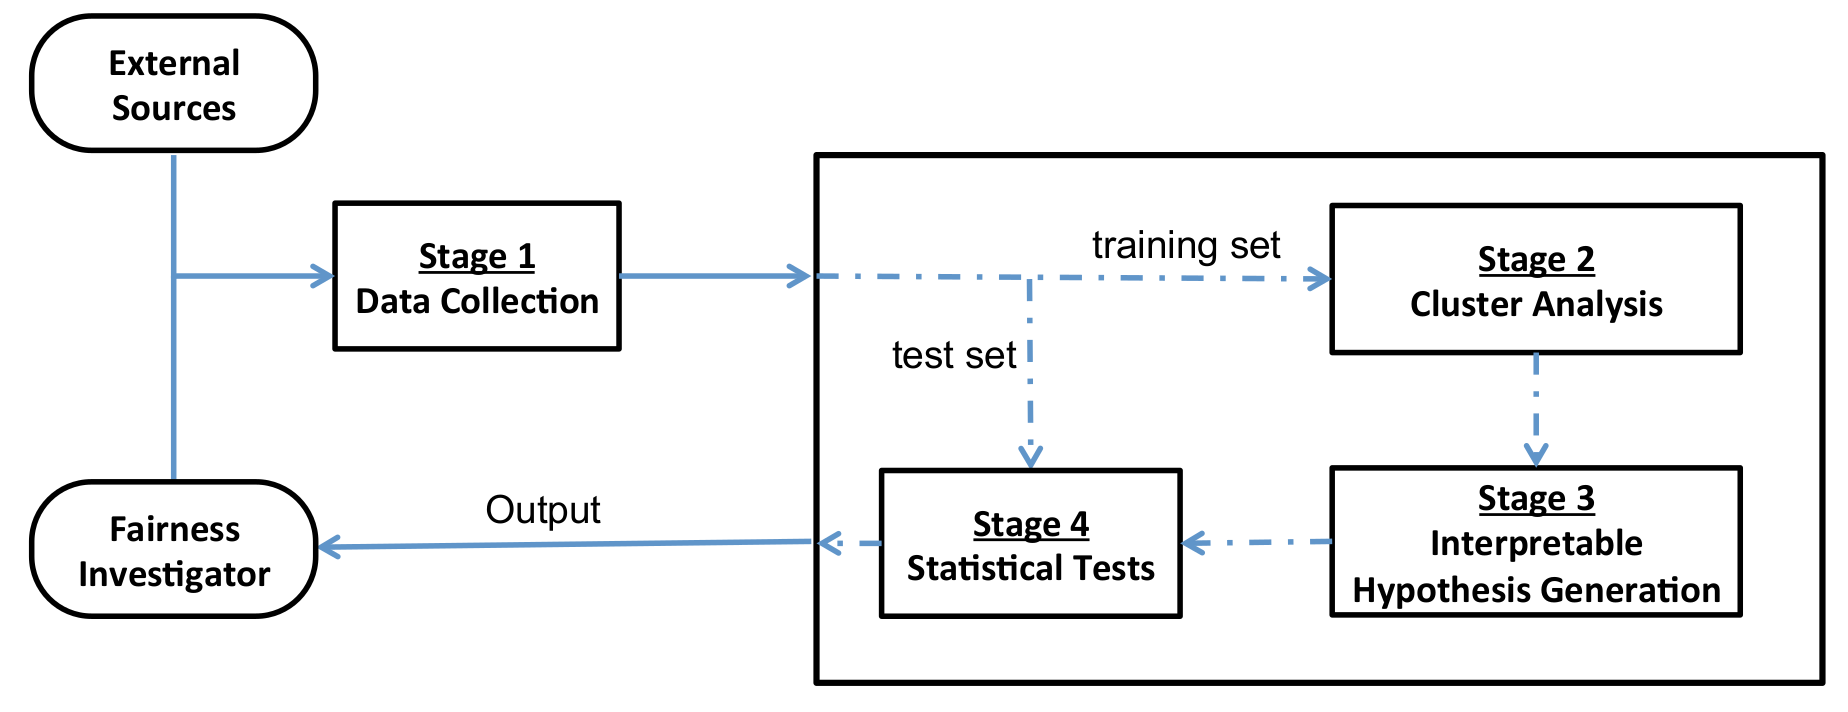
\includegraphics[width=\textwidth]{genericPipeline}
  \end{center}
  On a quatre étapes qui peuvent en théorie être effectuées indépendamment :
  \begin{description}[style=nextline]
  \item[1. Acquisition de donnée]
    étape consistant à mettre en forme le dataset, à le séparer en ensemble d'apprentissage et ensemble de test, à les traiter pour enlever les attributs protégés, en les sauvegardant dans un ensemble auxiliaire afin d'étudier ultérieurement les biais.

  \item[2. Partionnement de données et apprentissage]
    étape consistant à entraîer un classifieur approximant la décision prise sur l'ensemble d'entraînement pour pouvoir par la suite interpréter.

  \item[3. Génération d'hypothèse interprétable]
    étape consistant à formuler l'hypothèse nulle, dans notre cas qu'il n'y a pas de biais dans les groupes observés.

  \item[4. Tests statistiques]
    étape consistant à effectuer des mesures d'équité en fonction des hypothèses précédemment établies et à calculer les p-valeurs correspondantes.
  \end{description}

  Après ces quatre étapes, on doit rajouter une étape d'études des résultats statistiques pour déterminer s'il y a vraiment un biais et si on doit réitérer en modifiant le dataset.
\end{myRem}

\end{document}
